\documentclass{article}
\usepackage[spanish]{babel}
\usepackage{physics}
\usepackage{graphicx}

% Units Section %
%%%%%%%%%%%%%%%%%
\usepackage{siunitx}
\DeclareSIUnit{\angstrom}{\text{Å}}
\DeclareSIUnit{\calorie}{\text{cal}}
\DeclareSIUnit{\elementarycharge}{\text{\ensuremath{e}}}
\newcommand{\internationalUnitSystem}{\textnormal{si}}
\newcommand{\realUnitSystem}{\textnormal{re}}
\newcommand{\thermochemical}{\text{tq}}


\title{Movimiento de un electrón expuesto a un campo eléctrico constante}

\author{Pablo Brianese}

\begin{document}
  \maketitle
  \begin{abstract}
    Estudiamos el movimiento de un electrón expuesto a un campo eléctrico externo constante mediante la resolución analítica de las ecuaciones que gobiernan su movimiento.
    Compararemos los resultados obtenidos con las soluciones numéricas.  
  \end{abstract}

  \section{Sistema de unidades \texttt{real}}

  En el sistema de unidades \texttt{real} de LAMMPS
  \begin{itemize}
    \item La unidad de cantidad de sustancia es el mol.
    Un mol consiste de \(N = 6.022 140 76 \cdot 10^{23}\) partículas.
    Aquí \(N\) es el número de Avogadro, y la constante de Avogadro se define como \(N_A = N \unit{\per\mole}\).

    \item la unidad de masa es el gramo por mol, cuyo símbolo es \(\unit{\gram\per\mole}\).
    Esta unidad de masa no puede convertirse a los kilogramos del Sistema Internacional de Unidades.
    En cambio, procedemos interpretando que la medición de una masa \(m_{\unit{\kilogram}}\) en \(\unit{\kilogram}\) representa la masa de una partícula y la transformación a \(\unit{\gram\per\mole}\) consiste en responder a la pregunta
    ¿cuánta es \(m_{\unit{\gram\per\mole}}\), la masa por mol de una sustancia formada por partículas cada una de las cuales tiene individualmente masa \(m_{\unit{\kilo\gram}}\)?
    La respuesta es \(m_{\unit{\gram\per\mole}} = N 10^3 m_{\unit{\kilogram}}\).
%    Podríamos decir que \(\unit{\gram\per\mole} = N_A 10^{- 3} \unit{\kilogram}\).

    \item La unidad de distancia es el angstrom, cuyo símbolo es \(\unit{\angstrom}\), y verifica \(\unit{\angstrom} = 10^{- 10} \unit{\metre
    }\).

    \item La unidad de tiempo es el femtosegundo, cuyo símbolo es \(\unit{\femto\second}\), y verifica \(\unit{\femto\second} = 10^{- 15} s\).

    \item La unidad de energía es la kilocaloría por mol, cuyo símbolo es \(\unit{\kilo\calorie\per\mole}\).
    Definiendo una caloría como \(4.184 \unit{\joule}\) (la caloría termoquímica), resulta \(\unit{\kilo\calorie} = 4184 \unit{\joule}\).
    Esta unidad de energía no puede convertirse a los Julios del Sistema Internacional de Unidades.
    En cambio, procedemos interpretando que la medición de una energía \(\epsilon_{\unit{\joule}}\) en \(\unit{\joule}\) representa la energía de una partícula de tipo \(T\) y la transformación a \(\unit{\kilo\calorie\per\mole}\) y la transformación a \(\unit{\gram\per\mole}\) consiste en respondera la pregunta
    ¿cuánta es \(\epsilon_{\unit{\kilo\calorie\per\mole}}\), la energía por mol de una sustancia formada por partículas cada una de las cuales tiene individualmente energía \(\epsilon_{\unit{\joule}}\)?
    La respuesta es \(\epsilon_{\unit{\kilo\calorie\per\mole}} = N (4184)^{-1} \epsilon_{\unit{\joule}}\).

    \item La unidad de fuerza es la kilocaloría por mol--angstrom, cuyo símbolo es \(\unit{\kilo\calorie\per\mole\per\angstrom}\).
    Esta unidad de fuerza no puede convertirse a los Newtons del Sistema Internacional de Unidades.
    En cambio, procedemos interpretando que la medición de una fuerza \(f_{\unit{\newton}}\) en \(\unit{\newton}\) representa una fuerza externa aplicada sobre una partícula y la transformación a \(\unit{\kilo\calorie\per\mole\per\angstrom}\) consiste en responder a la siguiente pregunta
    ¿Cuál es \(f_{\unit{\kilo\calorie\per\mole\per\angstrom}}\), la fuerza que gobierna el movimiento del centro de masa de un mol de una sustancia formada por partículas cada una de las cuales sufre la acción de una fuerza externa igual a \(f_{\unit{\newton}}\)?
    La respuesta es \(f_{\unit{\kilo\calorie\per\mole\per\angstrom}} = N (4184)^{- 1} 10^{- 10} f_{\unit{\newton}}\).

    \item La unidad de carga eléctrica es la carga elemental (1.0 es un protón), cuyo símbolo es \(\unit{\elementarycharge}\), y verifica \(\unit{\elementarycharge} = 1.602 176 634 \cdot 10^{- 19} \unit{\coulomb}\).

    \item La unidad del campo eléctrico es el voltio por angstrom, cuyo símbolo es \(\unit{\volt\per\angstrom}\), y verifica \(\unit{\volt\per\angstrom} = 10^{- 10} \unit{\volt\per\metre}\).
  \end{itemize}

  Comparando con el Sistema Internacional de Unidades, obtenemos expresiones
  para la aceleración, usando la regla de la cadena
  \begin{align}
    \vec{a}_{\realUnitSystem}
    &=
    \frac{\dd^2 \vec{r}_{\realUnitSystem}}{\dd t_{\realUnitSystem}^2}
    =
    \frac{\dd}{\dd t_{\internationalUnitSystem}} \left( \frac{\dd \vec{r}_\realUnitSystem}{\dd t_{\internationalUnitSystem}} \frac{\dd t_{\internationalUnitSystem}}{\dd t_\realUnitSystem} \right) \frac{\dd t_{\internationalUnitSystem}}{\dd t_{\realUnitSystem}}
    =
    \frac{\dd}{\dd t_{\internationalUnitSystem}} \left( \frac{\dd \vec{r}_\realUnitSystem}{\dd t_{\internationalUnitSystem}} \frac{\unit{\second}}{\unit{\femto\second}} \right) \frac{\unit{\second}}{\unit{\femto\second}}
    =
    10^{- 30} \frac{\dd^2 \vec{r}_{\realUnitSystem}}{\dd t_{\internationalUnitSystem}^2}
    \\
    &=
    10^{- 30} \frac{\dd^2}{\dd t_{\internationalUnitSystem}^2} \frac{\unit{\metre}}{\unit{\angstrom}} \vec{r}_{\internationalUnitSystem}   % Angstrom = 10^{-10} metre -->  10^{- 10} l_Angstrom = l_metre
    =
    10^{- 20} \frac{\dd^2 \vec{r}_{\internationalUnitSystem}}{\dd t_{\internationalUnitSystem}^2}
    \\
    &=
    10^{- 20} \vec{a}_{\internationalUnitSystem}
  \end{align}

  \section{La Ley de Newton y la Fuerza de Lorentz}
  Como consecuencia de esta selección de unidades, la ley de Newton y la fuerza de Lorentz cambian de forma.
  Para hallar sus variantes partimos de sus expresiones conocidas en el Sistema Internacional de Unidades.
  La ley de Newton se escribe como
  \begin{align}
    \vec{F}_{\internationalUnitSystem} = m_{\internationalUnitSystem} \vec{a}_{\internationalUnitSystem}
  \end{align}
  Usando la ecuación
  \(
    m_{\realUnitSystem} = N_A 10^3 m_{\internationalUnitSystem}
  \)
  , deducimos
  \begin{align}
    N_A 10^3 \vec{F}_{\internationalUnitSystem}
    =
    m_{\realUnitSystem} \vec{a}_{\internationalUnitSystem}
  \end{align}
  Luego transformamos \(\vec{a}_{\internationalUnitSystem}\), mediante la ecuación
  \(
    \vec{a}_{\realUnitSystem} = 10^{- 20} \vec{a}_{\internationalUnitSystem}
  \),
  para obtener
  \begin{align}
    N_A 10^{- 20} 10^3 \vec{F}_{\internationalUnitSystem}
    =
    m_{\realUnitSystem} \vec{a}_{\realUnitSystem}
  \end{align}
  Finalmente, la igualdad \(\vec{F}_{\realUnitSystem} = N_A (4184)^{-1} 10^{- 10} \vec{F}_{\internationalUnitSystem}\) nos dá la verdadera forma de la ley de Newton en unidades \texttt{real}
  \begin{align}
    \vec{F}_{\realUnitSystem}
    =
    \frac{10^7}{4184} m_{\realUnitSystem} \vec{a}_{\realUnitSystem}
  \end{align}

  Por otro lado, dado que el campo magnético es idénticamente nulo, la fuerza de Lorentz toma (en el Sistema Internacional de Unidades) la forma
  \begin{align}
    \vec{F}_{\internationalUnitSystem}
    =
    q_{\internationalUnitSystem} \vec{E}_{\internationalUnitSystem}
  \end{align}
  La igualdad \(\vec{F}_{\realUnitSystem} = N (4184)^{-1} 10^{- 10} \vec{F}_{\internationalUnitSystem}\) nos lleva a
  \begin{align}
    \vec{F}_{\realUnitSystem}
    =
    \frac{N}{4184} 10^{- 10}
    q_{\internationalUnitSystem} \vec{E}_{\internationalUnitSystem}
  \end{align} 
  La definición del Coulombio nos permite decir que
  \begin{align}
    \vec{F}_{\realUnitSystem}
    =
    \frac{N c_p}{4184} 10^{- 10}
    q_{\realUnitSystem} \vec{E}_{\internationalUnitSystem}
  \end{align}
  donde \(c_p = 1.602 176 634 \cdot 10^{- 19}\) es el valor numérico de la carga en Coulombios de un protón (adimensional, como número puro).
  La ecuación para el campo eléctrico \(\vec{E}_{\internationalUnitSystem} = 10^{10} \vec{E}_{\realUnitSystem}\) nos da la fórmula para la fuerza de Lorentz en el sistema de unidades \texttt{real} de \texttt{lammps}
  \begin{align}
    \vec{F}_{\realUnitSystem}
    =
    \frac{N c_p}{4184}
    q_{\realUnitSystem} \vec{E}_{\realUnitSystem}
  \end{align}

  \section{Movimiento de un electrón expuesto a un campo eléctrico constante}
  Ahora podemos resolver las ecuaciones que gobiernan el movimiento de un electrón expuesto a un campo eléctrico externo en el sistema de unidades \texttt{real} de \texttt{lammps}.

  Una partícula de masa \(m \unit{\gram\per\mole}\) y carga \(q \unit{\elementarycharge}\) expuesta a un campo eléctrico \(\vec{E} \unit{\volt\per\angstrom}\) y a un campo magnético nulo, recibe la fuerza de Lorentz \(\vec{F} \unit{\kilo\calorie\per\mole\per\angstrom}\) dada por \(\vec{F} = N (4184)^{- 1} 10^{- 10} q \vec{E}\).
  Así, su movimiento queda determinado por la Ley de Newton \(\vec{F} = (4184)^{- 1} 10^7 m \vec{a}\), su posición inicial \(\vec{r}_0\) y su velocidad inicial \(\vec{v}_0\).
  La solución a este problema de valores iniciales puede derivarse, usando que el campo eléctrico es constante, como sigue
  \begin{align}
    10^7 (4184)^{- 1} m \vec{a}
      &=
      \vec{F}
    \\
    10^7 (4184)^{- 1} m \vec{a}
      &=
      N c_p (4184)^{- 1} q \vec{E}
    \\
    m \vec{a}
      &=
      N c_p 10^{-7} q \vec{E}
    \\
    m \vec{a}
      &=
      C q \vec{E}
    && C = N c_p 10^{-7}
    \\
    \vec{a}
      &=
      C \frac{q}{m} \vec{E}
    \\
    \frac{\dd \vec{v}}{\dd t}
      &=
      C \frac{q}{m} \vec{E}
      \quad\leftarrow \text{no depende de } t
    \\
    \vec{v}
      &=
      C \frac{q}{m} \vec{E} \cdot t + \vec{v}_0
    \\
    \frac{\dd \vec{r}}{\dd t}
      &=
      C \frac{q}{m} \vec{E} \cdot t + \vec{v}_0
    \\
    \vec{r}
      &=
      C \frac{q}{m} \vec{E} \cdot \frac{t^2}{2} + \vec{v}_0 \cdot t + \vec{r}_0
  \end{align}

  A tiempo \(t = 0\), la partícula parte de la posición \(\vec{r}_0 = (0, 0, 100)\) con una velocidad \(\vec{v}_0 = (10, 0, 0)\).
  El campo electrico está dirigido en el sentido positivo del eje \(y\), con una intensidad de \(0.1\).
  Lo que es decir, el campo electrico externo es constantemente \(\vec{E} = (0, 10^{- 1}, 0)\).
  La masa del electrón es \(m = 0.00054854 \unit{\gram\per\mole}\) y su carga es \(q = - 1 \unit{\elementarycharge}\).
  Con esta información podemos graficar la expresión analítica que obtuvimos para la posición del electrón.

  \newpage
  \section{Gráficas}
  \begin{figure}[h!]
    \includegraphics
      [width=\textwidth]
      {../lammps/dat/electronEnCampoElectrico.png}
    \caption{Traza del movimiento de un electrón. Resultado de la simulación con LAMMPS.}
  \end{figure}

  \begin{figure}
    \includegraphics
    [width=\textwidth]
    {../python/scipy/dat/electronEnCampoElectrico.png}
    \caption{Traza del movimiento de un electrón. Resultado de la integración con SciPy.}
  \end{figure}

  \begin{figure}
    \includegraphics
  [width=\textwidth]
  {../python/solucion_analitica/dat/electronEnCampoElectrico.png}
    \caption{Traza del movimiento de un electrón. Resultado de la solución analítica}
  \end{figure}
\end{document}